% HEADER
\noindent
{\bfseries\sffamily\fontsize{10}{12}\selectfont 280}\hspace{2.5em}%
{\bfseries\sffamily\fontsize{9}{11}\selectfont\color{stewartteal} CHƯƠNG 4}\hspace{1.5em}%
{\sffamily\fontsize{9}{11}\selectfont\color{stewartteal} Ứng dụng của Đạo hàm}

\vspace{10pt}

% SECTION TITLE ROW
\noindent
\begin{minipage}[c]{48mm}
  \raggedleft
  \begin{tikzpicture}[baseline={(0,0.6)}]
    \foreach \i in {0, 2.5, 5.0, 7.5, 10.0} {
      \draw[line width=0.8pt, color=cyanrule] (0, \i pt) -- (34pt, \i pt);
    }
  \end{tikzpicture}\hspace{8pt}%
  {\fontsize{24}{26}\selectfont\bfseries\color{stewartteal} 4.1}\hspace{8pt}%
  {\color{stewartteal}\rule[-4pt]{1.2pt}{24pt}}%
\end{minipage}%
\hspace{6mm}%
\begin{minipage}[c]{131mm}
  {\fontsize{18}{22}\selectfont\bfseries\sffamily Giá trị lớn nhất và Giá trị nhỏ nhất}
\end{minipage}

\vspace{10pt}

% TWO-COLUMN BODY
\noindent
\begin{minipage}[t]{48mm}
  % FIGURE 1 (dóng hàng với mục Cực trị)
  \vspace*{50mm}
  \noindent
  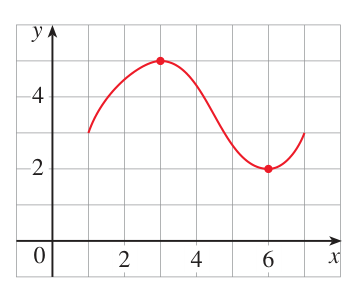
\includegraphics[width=\linewidth]{images/p0315_fig1.png}\\[3pt]
  {\bfseries\sffamily\fontsize{8.5}{10}\selectfont HÌNH 1}

  % FIGURE 2 (dóng hàng với đoạn văn bản Hình 2)
  \vspace{16mm}
  \noindent
  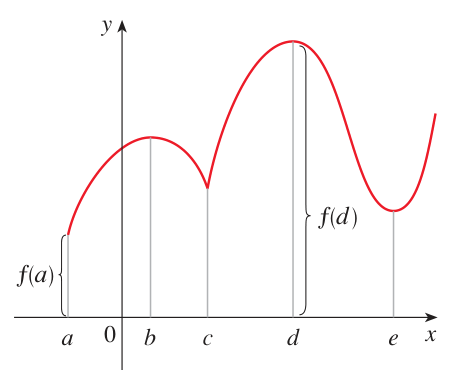
\includegraphics[width=\linewidth]{images/p0315_fig2.png}\\[3pt]
  {\bfseries\sffamily\fontsize{8.5}{10}\selectfont HÌNH 2}\\[2pt]
  {\fontsize{7.5}{9}\selectfont Cực tiểu tuyệt đối $f(a)$, cực đại tuyệt đối $f(d)$, cực tiểu địa phương $f(c), f(e)$, cực đại địa phương $f(b), f(d)$}

  % FIGURE 3 (dóng hàng với đoạn văn bản Hình 3)
  \vspace{14mm}
  \noindent
  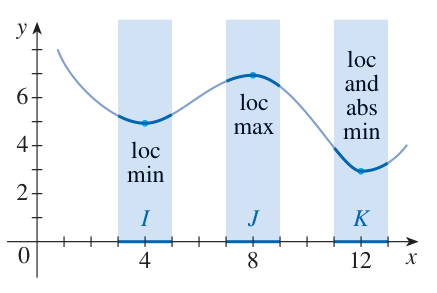
\includegraphics[width=\linewidth]{images/p0315_fig3.png}\\[3pt]
  {\bfseries\sffamily\fontsize{8.5}{10}\selectfont HÌNH 3}
\end{minipage}%
\hfill
\begin{minipage}[t]{131mm}
  \noindent
  Một trong những ứng dụng quan trọng nhất của phép tính vi phân là các \emph{bài toán tối ưu hóa}, trong đó chúng ta được yêu cầu tìm cách tối ưu (tốt nhất) để thực hiện một việc gì đó. Dưới đây là các ví dụ về những bài toán như vậy mà chúng ta sẽ giải quyết trong chương này:

  \begin{itemize}[leftmargin=1.2em, itemsep=2pt, topsep=3pt, parsep=0pt]
    \item[\textcolor{defred}{\textbullet}] Hình dạng của một chiếc vỏ lon như thế nào sẽ tối thiểu hóa chi phí sản xuất?
    \item[\textcolor{defred}{\textbullet}] Gia tốc cực đại của một tàu vũ trụ là bao nhiêu? (Đây là một câu hỏi quan trọng đối với các phi hành gia, những người phải chịu đựng tác động của gia tốc.)
    \item[\textcolor{defred}{\textbullet}] Bán kính của khí quản bị co lại là bao nhiêu để tống không khí ra ngoài nhanh nhất khi ho?
    \item[\textcolor{defred}{\textbullet}] Các mạch máu nên phân nhánh ở góc bao nhiêu để giảm thiểu năng lượng mà tim tiêu hao khi bơm máu?
  \end{itemize}

  \vspace{3pt}
  \noindent
  Những bài toán này có thể quy về việc tìm giá trị lớn nhất hoặc giá trị nhỏ nhất của một hàm số. Trước hết, hãy giải thích chính xác ý nghĩa của giá trị lớn nhất và giá trị nhỏ nhất.

  \vspace{8pt}
  \noindent
  {\color{stewartteal}\blacksquare}\hspace{0.5em}{\bfseries\sffamily Giá trị cực trị tuyệt đối và địa phương}

  \vspace{3pt}
  \noindent
  Ta thấy rằng điểm cao nhất trên đồ thị của hàm số $f$ được chỉ ra trong Hình~1 là điểm $(3, 5)$. Nói cách khác, giá trị lớn nhất của $f$ là $f(3) = 5$. Tương tự, giá trị nhỏ nhất là $f(6) = 2$. Ta nói rằng $f(3) = 5$ là \emph{cực đại tuyệt đối} của $f$ và $f(6) = 2$ là \emph{cực tiểu tuyệt đối}. Tổng quát, chúng ta sử dụng định nghĩa sau đây.

  \vspace{5pt}
  \begin{stewartbox}
  \noindent
  \tikz[baseline=(N.base)]{\node[draw=defred, line width=0.8pt, fill=white, text=defred, font=\bfseries\sffamily\fontsize{9.5}{10}\selectfont, inner sep=2pt, rounded corners=1.5pt] (N) {1};}\hspace{6pt}%
  {\bfseries\sffamily\color{defred}\fontsize{10}{11}\selectfont Định nghĩa}\hspace{8pt}%
  Cho $c$ là một số thuộc tập xác định $D$ của hàm số $f$. Khi đó $f(c)$ là
  \begin{itemize}[leftmargin=1.5em, itemsep=2pt, topsep=3pt, parsep=0pt]
    \item[\textcolor{defred}{\textbullet}] \textbf{giá trị cực đại tuyệt đối} của $f$ trên $D$ nếu $f(c) \geqslant f(x)$ với mọi $x \in D$.
    \item[\textcolor{defred}{\textbullet}] \textbf{giá trị cực tiểu tuyệt đối} của $f$ trên $D$ nếu $f(c) \leqslant f(x)$ với mọi $x \in D$.
  \end{itemize}
  \end{stewartbox}

  \vspace{4pt}
  \noindent
  Một cực đại tuyệt đối hoặc cực tiểu tuyệt đối đôi khi được gọi là cực đại hoặc cực tiểu \textbf{toàn cục}. Các giá trị lớn nhất và nhỏ nhất của $f$ được gọi là các \textbf{giá trị cực trị} của $f$.

  Hình~2 minh họa đồ thị của một hàm số $f$ với cực đại tuyệt đối tại $d$ và cực tiểu tuyệt đối tại $a$. Lưu ý rằng $(d, f(d))$ là điểm cao nhất trên đồ thị và $(a, f(a))$ là điểm thấp nhất. Trong Hình~2, nếu chúng ta chỉ xét các giá trị của $x$ ở gần $b$ [chẳng hạn, nếu chúng ta giới hạn sự chú ý của mình trong khoảng $(a, c)$], thì $f(b)$ là giá trị lớn nhất trong số các giá trị đó của $f(x)$ và được gọi là một \emph{giá trị cực đại địa phương} của $f$. Tương tự, $f(c)$ được gọi là một \emph{giá trị cực tiểu địa phương} của $f$ vì $f(c) \leqslant f(x)$ khi $x$ ở gần $c$ [chẳng hạn trong khoảng $(b, d)$]. Hàm số $f$ cũng có một cực tiểu địa phương tại $e$. Tổng quát, chúng ta có định nghĩa sau đây.

  \vspace{5pt}
  \begin{stewartbox}
  \noindent
  \tikz[baseline=(N.base)]{\node[draw=defred, line width=0.8pt, fill=white, text=defred, font=\bfseries\sffamily\fontsize{9.5}{10}\selectfont, inner sep=2pt, rounded corners=1.5pt] (N) {2};}\hspace{6pt}%
  {\bfseries\sffamily\color{defred}\fontsize{10}{11}\selectfont Định nghĩa}\hspace{8pt}%
  Số $f(c)$ là một
  \begin{itemize}[leftmargin=1.5em, itemsep=2pt, topsep=3pt, parsep=0pt]
    \item[\textcolor{defred}{\textbullet}] \textbf{giá trị cực đại địa phương} của $f$ nếu $f(c) \geqslant f(x)$ khi $x$ ở gần $c$.
    \item[\textcolor{defred}{\textbullet}] \textbf{giá trị cực tiểu địa phương} của $f$ nếu $f(c) \leqslant f(x)$ khi $x$ ở gần $c$.
  \end{itemize}
  \end{stewartbox}

  \vspace{4pt}
  \noindent
  Trong Định nghĩa 2 (và ở những nơi khác), nếu chúng ta nói rằng một điều gì đó đúng \textbf{ở gần} $c$, chúng ta muốn nói rằng nó đúng trên một khoảng mở nào đó chứa $c$. (Do đó, một cực đại hoặc cực tiểu địa phương không thể xảy ra tại một điểm mút.) Chẳng hạn, trong Hình~3 chúng ta thấy rằng $f(4) = 5$ là một cực tiểu địa phương vì nó là giá trị nhỏ nhất của $f$ trên khoảng $I$. Nó không phải là cực tiểu tuyệt đối vì $f(x)$ nhận các giá trị nhỏ hơn khi $x$ ở gần 12 (chẳng hạn trong khoảng $K$). Trên thực tế $f(12) = 3$ vừa là một cực tiểu địa phương vừa là cực tiểu tuyệt đối. Tương tự, $f(8) = 7$ là một cực đại địa phương, nhưng không phải là cực đại tuyệt đối vì $f$ nhận các giá trị lớn hơn khi ở gần 1.
\end{minipage}

% FOOTER
\vfill
\noindent
\begin{minipage}{\textwidth}
  \centering
  \fontsize{6.5}{8}\selectfont\color{gray!80!black}
  Copyright 2021 Cengage Learning. All Rights Reserved. May not be copied, scanned, or duplicated, in whole or in part. WCN 02-200-203\\[2pt]
  Due to electronic rights, some third party content may be suppressed from the eBook and/or eChapter(s). Editorial review has deemed that any suppressed content does not materially affect the overall learning experience. Cengage Learning reserves the right to remove additional content at any time if subsequent rights restrictions require it.
\end{minipage}
